\let\negmedspace\undefined
\let\negthickspace\undefined
\documentclass[journal]{IEEEtran}
\usepackage[a5paper, margin=10mm, onecolumn]{geometry}
%\usepackage{lmodern} % Ensure lmodern is loaded for pdflatex
\usepackage{tfrupee} % Include tfrupee package

\setlength{\headheight}{1cm} % Set the height of the header box
\setlength{\headsep}{0mm}  % Set the distance between the header box and the top of the text

\usepackage{gvv-book}
\usepackage{gvv}
\usepackage{cite}
\usepackage{amsmath,amssymb,amsfonts,amsthm}
\usepackage{algorithmic}
\usepackage{graphicx}
\usepackage{textcomp}
\usepackage{xcolor}
\usepackage{txfonts}
\usepackage{listings}
\usepackage{enumitem}
\usepackage{mathtools}
\usepackage{gensymb}
\usepackage{comment}
\usepackage[breaklinks=true]{hyperref}
\usepackage{tkz-euclide} 
\usepackage{listings}
% \usepackage{gvv}                                        
\def\inputGnumericTable{}                                 
\usepackage[latin1]{inputenc}                                
\usepackage{color}                                            
\usepackage{array}                                            
\usepackage{longtable}                                       
\usepackage{calc}                                             
\usepackage{multirow}                                         
\usepackage{hhline}                                           
\usepackage{ifthen}                                           
\usepackage{lscape}
\usepackage{tikz}
\usetikzlibrary{patterns}
\begin{document}

\bibliographystyle{IEEEtran}
\vspace{3cm}

\title{2008-CE- 35-51}
\author{EE24BTECH11021 - Eshan Ray}

% \maketitle
% \newpage
% \bigskip
{\let\newpage\relax\maketitle}

\renewcommand{\thefigure}{\theenumi}
\renewcommand{\thetable}{\theenumi}
\setlength{\intextsep}{10pt} % Space between text and floats

\begin{enumerate}
\setcounter{enumi}{34}
    \item The span\brak{s} to be loaded uniformly for maximum positive \brak{upward} reaction at support $P$, as shown in the figure below, is\brak{are}

\begin{tikzpicture}

% Define coordinates for easier positioning
\coordinate (P) at (0,0);
\coordinate (Q) at (3,0);
\coordinate (R) at (6,0);
\coordinate (S) at (9,0);
\coordinate (T) at (3,-3);

% Draw the horizontal bar
\draw[thick] (P) -- (S);

% Draw the downward triangles
\draw (0,0) -- (0.4,-0.4) -- (-0.4,-0.4) -- cycle;

\draw (6,0) -- (6.4,-0.4) -- (5.6,-0.4) -- cycle;
\draw (9,0) -- (9.4,-0.4) -- (8.6,-0.4) -- cycle;

% Draw the vertical line and the shaded rectangle
\draw[thick] (Q) -- (T);
\fill[pattern=north east lines] (2.5,-3) rectangle (3.5,-3.5);
\fill[pattern=north east lines] (-0.5,-0.4) rectangle (0.5,-1);
\draw (-0.5,-0.4) -- (0.5,-0.4);
\draw (2.5,-3) -- (3.5,-3);
\draw (6.5,-0.6) -- (5.5,-0.6);
\draw (9.5,-0.6) -- (8.5,-0.6);
% Add small circles to the triangle sides at R and S
\draw (6.2,-0.5) circle (0.1cm);
\draw (5.8,-0.5) circle (0.1cm);
\draw (9.2,-0.5) circle (0.1cm);
\draw (8.8,-0.5) circle (0.1cm);

% Add labels
\node[above] at (P) {P};
\node[above] at (Q) {Q};
\node[above] at (R) {R};
\node[above] at (S) {S};
\node[below] at (T) {T};

\end{tikzpicture}



    \begin{enumerate}
        \item $PQ$ only
        \item $PQ$ and $PR$
        \item $QR$ and $RS$
        \item $PQ$ and $RS$
    \end{enumerate}
    \item A vertical rod $PQ$ of length $L$ is fixed at its top end $P$ and has a flange fixed to the bottom end $Q$. A weight $W$ is dropped vertically from a height $h\brak{\textless L}$ on to the flange. The axial stress in the rod can be reduced by
    \begin{enumerate}
        \item increasing the length of the rod 
        \item decreasing the length of the rod
        \item decreasing the area of cross-section of the rod
        \item increasing the modulus of elasticity of the material
    \end{enumerate}
    \item Un-factored maximum bending moments at a section of a reinforced concrete beam resulting from a frame analysis are $50,80,120\,and\,180\,kNm$ under dead, live, wind and earthquake loads respectively. The design moment \brak{kNm} as per $IS\colon456-2000$ for the limit state of collapse\brak{flexure} is
    \begin{enumerate}
        \item $195$
        \item $250$
        \item $345$
        \item $372$
    \end{enumerate}
    \item A reinforced concrete column contains longitudinal steel equals to $1$ percent of net cross-sectional area of the column. Assume modular ratio as $10$. The loads carried \brak{using\,the\,elastic\,theory} by the longitudinal steel and the net area of concrete, are $P_s$ and $P_c$ respectively. The ratio $\frac{P_s}{P_c}$ expressed as percent is
    \begin{enumerate}
        \item $0.1$
        \item $1$
        \item $1.1$
        \item $10$
    \end{enumerate}
    \item A pre-tensioned concrete member of section $200\,mm\times250\,mm$ contains tendons of area $500\,mm^2$ at centre of gravity of the section. The prestress in the tendons is $1000\,N/mm^2$. Assuming modular ratio as $10$, the stress \brak{N/mm^2} in concrete is 
    \begin{enumerate}
        \item $11$
        \item $9$
        \item $7$
        \item $5$
    \end{enumerate}
    \item Rivets and bolts subjected to both shear stress $\brak{\tau_{vf,cal}}$ and axial tensile stress $\brak{\sigma_{tf,cal}}$ shall be so proportioned that the stresses don not exceed the respective allowable stresses $\tau_{vf}$ and $\sigma_{tf}$ and the value of $\brak{\frac{\tau_{vf,cal}}{\tau_{vf}}+\frac{\sigma_{tf,cal}}{\sigma_{tf}}}$ does not exceed
    \begin{enumerate}
        \item $1.0$
        \item $1.2$
        \item $1.4$
        \item $1.8$
    \end{enumerate}
    \item A continuous beam is loaded as shown in the figure below. Assuming a plastic moment capacity equal to $M_p$, the minimum load at which the beam would collapse is

  \begin{tikzpicture}

% Define coordinates for easier positioning
\coordinate (G) at (0,0);
\coordinate (H) at (2,0);
\coordinate (I) at (6,0);
\coordinate (J) at (10,0);
\coordinate (P1) at (4,1);
\coordinate (P2) at (8,1);

% Draw the horizontal bar
\draw[thick] (G) -- (J);

% Draw the downward triangles
\draw (0,0) -- (0.5,-0.4) -- (-0.5,-0.4) -- cycle;
\draw (2,0) -- (2.5,-0.4) -- (1.5,-0.4) -- cycle;
\draw (6,0) -- (6.5,-0.4) -- (5.5,-0.4) -- cycle;
\draw (10,0) -- (10.5,-0.4) -- (9.5,-0.4) -- cycle;

% Draw the vertical lines and arrows
\draw[thick,->] (P1) -- (4,0);
\draw[thick,->] (P2) -- (8,0);

% Add labels
\node[above] at (G) {G};
\node[above] at (H) {H};
\node[above] at (I) {I};
\node[above] at (J) {J};
\node[above] at (P1) {P};
\node[above] at (P2) {P};

% Add length labels with lines
\draw (-0.5,-0.7) -- (2,-0.7) node[midway, below] {L};
\draw (2,-0.7) -- (4,-0.7) node[midway, below] {L/2};
\draw (4,-0.7) -- (6,-0.7) node[midway, below] {L/2};
\draw (6,-0.7) -- (8,-0.7) node[midway, below] {L/2};
\draw (8,-0.7) -- (10.5,-0.7) node[midway, below] {L/2};
\draw[thick] (2,-0.5) -- (2,-0.9);
\draw[thick] (4,-0.5) -- (4,-0.9);
\draw[thick] (6,-0.5) -- (6,-0.9);
\draw[thick] (8,-0.5) -- (8,-0.9);
\draw[thick] (10,-0.5) -- (10,-0.9);
\draw[thick] (0,-0.5) -- (0,-0.9);
\end{tikzpicture}

    \begin{enumerate}
        \item $\frac{4M_p}{L}$
        \item $\frac{6M_p}{L}$
        \item $\frac{8M_p}{L}$
        \item $\frac{10M_p}{L}$
    \end{enumerate}
    \item The maximum tensile stress at the section $X-X$ shown in the figure below is 

    \begin{tikzpicture}

% Define coordinates for easier positioning
\coordinate (A) at (0,0);
\coordinate (B) at (2,0);
\coordinate (C) at (2,-0.5);
\coordinate (D) at (4,-0.5);
\coordinate (E) at (4,0);
\coordinate (F) at (6,0);
\coordinate (G) at (6,-1);
\coordinate (H) at (0,-1);
% Draw the horizontal bar
\draw[thick] (A) -- (B);
\draw[thick] (C) -- (D);
\draw[thick] (E) -- (F);
\draw[thick] (G) -- (H);
\draw[thick] (0,0.25)-- (0,-1.25);
\draw[thick] (0,1)--(6,1);
\draw[thick] (0,1.25)--(0,0.75);
\draw[thick] (6,1.25)--(6,0.75);
\draw[thick] (2,1.25)--(2,0.75);
\draw[thick] (4,1.25)--(4,0.75);
% Draw the vertical lines
\draw (A) -- (H);
\draw (B) -- (C);
\draw (D) -- (E);
\draw (F) -- (G);

% Add labels for L/3
\node[above] at (1,1) {L/3};
\node[above] at (3,1) {L/3};
\node[above] at (5,1) {L/3};

% Draw the shaded rectangle
\fill[pattern=north east lines] (0,0.25) rectangle (-1,-1.25);

% Draw the horizontal line with arrow
\draw (7,0) -- (7,-0.5) node[midway, right] {d/2};

% Draw the vertical line and arrow
\draw (7,-0.5) -- (7,-1) node[midway, right] {d/2};

% Draw the rectangle
\draw (9,0) rectangle (9.5,-1);
\node[above] at (9.25,0) {b};
\node[right] at (9.5,-0.5) {d};
% Add labels for L/2
\node[below] at (1.5,-1.5) {L/2};
\node[below] at (4.5,-1.5) {L/2};
\draw[<->] (0.05,-1.5)--(2.9,-1.5);
\draw[<->] (3.1,-1.5)--(5.95,-1.5);
\draw[thick] (0,-1.35)--(0,-1.65);
\draw[thick] (2.9,-1.35)--(2.9,-1.65);
\draw[thick] (3.1,-1.35)--(3.1,-1.65);
\draw[thick] (6,-1.35)--(6,-1.65);
\draw[thick] (7,0.1)--(7,-1.1);
\draw[thick] (6.9,0)--(7.1,0);
\draw[thick] (6.9,-1)--(7.1,-1);
% Add label for X
\node[below] at (3,-1.6) {X};
\node[above] at (3,0.5) {X};
\draw[dashed] (3,-1.6)--(3,0.5);
\draw[dashed] (4,-0.5)--(6,-0.5);
\draw[->] (6,-0.5)--(8,-0.5);
\end{tikzpicture}
    \begin{enumerate}
        \item $\frac{8P}{bd}$
        \item $\frac{6P}{bd}$
        \item $\frac{4P}{bd}$
        \item $\frac{2P}{bd}$
    \end{enumerate}
    \item The stepped cantilever is subjected to moments, $M$ as shown in the figure below. The vertical deflection at the free end\brak{neglecting\, the\,self\,weight} is

    
\begin{tikzpicture}

% Define coordinates for easier positioning
\coordinate (A) at (0,0);
\coordinate (B) at (2,0);
\coordinate (C) at (2,-0.5);
\coordinate (D) at (4,-0.5);
\coordinate (E) at (4,-1);
\coordinate (F) at (0,-1);
% Draw the horizontal bar
\draw[thick] (A) -- (B);
\draw[thick] (C) -- (D);
\draw[thick] (F) -- (E);
\draw[thick] (B) -- (C);
\draw[thick] (D) -- (E);
\draw[thick] (A) -- (F);
% Draw the shaded rectangle
\fill[pattern=north east lines] (0,0.25) rectangle (-1,-1.25);

% Add labels for 2EI and EI
\node[below] at (1,-0.25) {2EI};
\node[above] at (3.1,-0.5) {EI};

% Add labels for L/2
\node[below] at (1,-1.75) {L/2};
\node[below] at (3,-1.75) {L/2};
\draw[thick] (-0.25,-1.75)--(4.25,-1.75);
\draw[thick] (0,-1.5)--(0,-2);
\draw[thick] (2,-1.5)--(2,-2);
\draw[thick] (4,-1.5)--(4,-2);
% Draw the arrows and moment labels
\draw[->] (2.05,-1.2) arc (-90:90:0.6);
\node[above] at (1.8,0) {M};
\draw[->] (4.2,0) arc (90:270:0.6);
\node[right] at (4.2,-1.2) {M};

\end{tikzpicture}
        \begin{enumerate}
            \item $\frac{ML^2}{8EI}$
            \item $\frac{ML^2}{4EI}$
            \item $\frac{ML^2}{2EI}$
            \item zero
        \end{enumerate}
    \item The liquid limit $\brak{LL}$, plastic limit $\brak{PL}$ and shrinkage limit $\brak{SL}$ of a cohesive soil satisfy the relation
        \begin{enumerate}
            \item $LL\textgreater PL\textless SL$
            \item $LL\textgreater PL\textgreater SL$
            \item $LL\textless PL\textless SL$
            \item $LL\textless PL\textgreater SL$
        \end{enumerate}
    \item A footing $2\,m\times1\,m$ exert a uniform pressure of $150\,kN/m^2$ on the soil. Assuming a load dispersion of $2$ vertical to $1$ horizontal, the average vertical stress $\brak{kN/m^2}$ at $1.0\,m$ below the footing is 
    \begin{enumerate}
        \item $50$
        \item $75$
        \item $80$
        \item $100$
    \end{enumerate}
    \item A direct shear test was conducted on a cohesionless soil $\brak{c=0}$ specimen under a normal stress of $200\,kN/m^2$. The specimen failed at a shear stress of $100\,kN/m^2$. The angle of internal friction of the soil $\brak{degrees}$ is
    \begin{enumerate}
        \item $26.6$
        \item $29.5$
        \item $30.0$
        \item $32.6$
    \end{enumerate}
    \item A pile of $0.50\,m$ diameter and of length $10\,m$ is embedded in a deposit of clay. The undrained strength parameters of the clay are cohesion$\,= 60\,kN/m^2$ and the angle of internal friction $=\,0$. The skin friction capacity $\brak{kN}$ of the pile for an adhesion factor of $0.6$, is
    \begin{enumerate}
        \item $671$
        \item $565$
        \item $283$
        \item $106$
    \end{enumerate}
    \item A saturated clay stratum draining both at the top and bottom undergoes $50$ percent consolidation in $16$ years under an applied load. If an additional drainage layer were present at the middle of the clay stratum, $50$ percent consolidation would occur in 
    \begin{enumerate}
        \item $2$ years
        \item $4$ years
        \item $8$ years
        \item $16$ years
    \end{enumerate}
    \item A test plate $30\,cm\times 30\,cm$ resting on a sand deposit settles by $10\,mm$ under a certain loading intensity. A footing $150\,cm\times 200\,cm$ resting on the same sand deposit and loaded to the same load intensity settles by
    \begin{enumerate}
        \item $2.0\,mm$
        \item $27.8\,mm$
        \item $30.2\,mm$
        \item $50.0\,mm$
    \end{enumerate}
    \item A volume of $3.0\times 10^6\,m^3$ of groundwater was pumped out from an unconfined aquifer uniformly from an area of $5\,km^2$. The pumping lowered the water table from initial level of $102\,m$ to $99\,m$. The specific yield of the aquifer is
    \begin{enumerate}
        \item $0.20$
        \item $0.30$
        \item $0.40$
        \item $0.50$
    \end{enumerate}
    \item A weir on a permeable foundation with downstream sheet pile is shown in the figure below. The exit gradient as per Khosla's method is 
    \begin{circuitikz}[scale=0.8]
\tikzstyle{every node}=[font=\normalsize]
\draw (6.5,10.25) to[short] (19.5,10.25);
\draw (17.25,10.25) to[short] (17.25,8.25);
\draw (12.75,10.25) to[short] (12.75,12.25);
\draw (12.75,12) to[short] (10.5,12);
\draw [<->, >=Stealth] (8.25,9.5) -- (17.25,9.5);
\draw (11.25,12) to[short] (9.5,12);
\draw (10.75,12) to[short] (10.25,12.5);
\draw (10.25,12.5) to[short] (11,12.5);
\draw (10.75,12) to[short] (11.25,12.5);
\draw (11.25,12.5) to[short] (10.75,12.5);
\draw (10.5,12) to[short] (11.25,12);
\draw (10.5,12) to[short] (11,12);
\draw (11,12) to[short] (10,12);
\draw (10,12) to[short] (11,12);
\draw (10.5,12) to[short] (11.25,12);
\draw (11.25,12) to[short] (9.75,12);
\draw (10.5,12) to[short] (11.25,12);
\draw (11.25,12) to[short] (10.25,12);
\draw (10.25,12) to[short] (11.25,12);
\draw [short] (13.25,12) -- (14,12);
\draw [<->, >=Stealth] (13.75,12) -- (13.75,10.25);
\draw [->, >=Stealth] (13.5,12.5) -- (12.75,11.5);
\draw [->, >=Stealth] (15.5,11.25) -- (15,10.25);
\draw (10.75,12.5) to (10.75,12.25) node[ground]{};
\draw (18.25,10.75) to (18.25,10.5) node[ground]{};
\draw [short] (18.25,10.75) -- (18.75,10.75);
\draw [short] (18.75,10.75) -- (18.25,10.25);
\draw [short] (18.25,10.25) -- (17.75,10.75);
\draw [short] (18.25,10.75) -- (17.75,10.75);
\draw [->, >=Stealth] (15.5,9) -- (17.25,9);
\draw [<->, >=Stealth] (17.75,10.25) -- (17.75,8.25);
\draw [short] (17.5,8.25) -- (18,8.25);
\draw [short] (8.25,9.75) -- (8.25,9.25);
\node [font=\normalsize] at (14,12.75) {Weir};
\node [font=\normalsize] at (16,11.5) {Floor};
\node [font=\normalsize] at (14.5,9.25) {Downstream};
\node [font=\normalsize] at (14.5,8.9) {Sheet pile};
\node [font=\normalsize] at (14.25,11.25) {5 m};
\node [font=\normalsize] at (18.25,9.25) {4 m};
\node [font=\normalsize] at (12.25,9.25) {10 m};
\end{circuitikz}

            \begin{enumerate}
                \item $1\,in\,6.0$
                \item $1\,in\,5.0$
                \item $1\,in\,3.4$
                \item $1\,in\,2.5$
            \end{enumerate}
\end{enumerate}
\end{document}
